\begin{flushleft}
  {\fontsize{12}{0} \bf 資料準備}
  \begin{abstract}
    \\\hspace{2em}
    本研究使用3000張黑白一整塊的PCB影像作為資料集\cite{deep_pcb_dataset},每張影像均包含瑕疵(defect)與無瑕疵(good)兩種版本。根據資料集的特性,對同一塊PCB影像中帶有瑕疵與無瑕疵的相同區域進行裁切,提取出多個小區塊,標註為瑕疵類別或無瑕疵類別。一張PCB影像可以裁切出多個小區塊,經過資料處理後,最終生成約20000張裁切的PCB區塊影像,作為訓練分類模型的資料來源。
    \\\hspace{2em}
    針對數量較少的瑕疵類別,透過資料增強技術進行平衡處理,包括旋轉、翻轉、添加高斯雜訊以及模擬光源變化等操作,以使各類別的樣本數量達到均衡。
    \\\hspace{2em}
    最終,模型的訓練任務為區塊分類,分類模型需辨識出6種類別的瑕疵(copper、mousebite、open、pin-hole、short、spur)以及1類無瑕疵的區塊(good),以實現高準確率的瑕疵檢測目標。
    黑白PCB資料集。
  \end{abstract}
  \begin{figure}[!hbp] 
    \centering 
    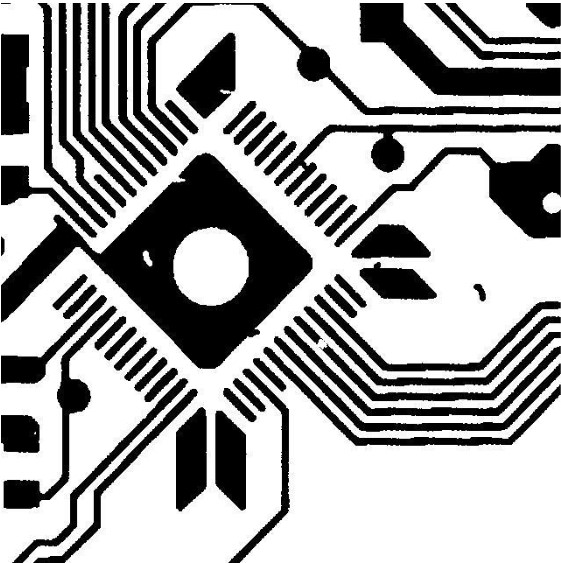
\includegraphics[width=0.65\linewidth, height=5cm]{img/defect_whole_pcb.jpg} 
    \caption{帶有瑕疵的黑白PCB影像}
    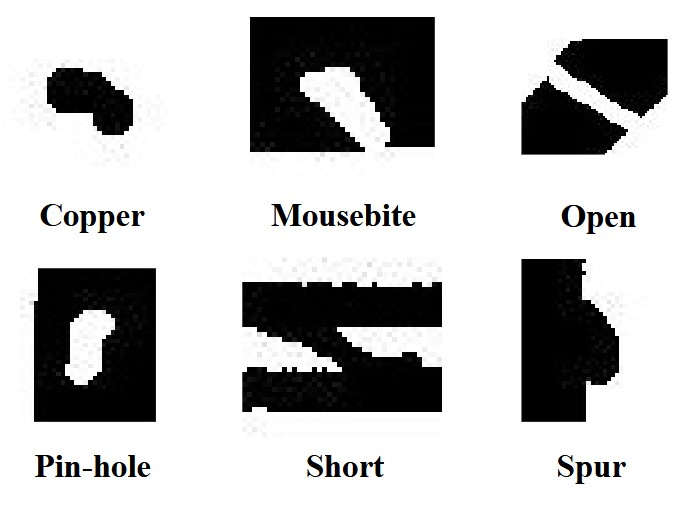
\includegraphics[width=0.85\linewidth, height=5.5cm]{img/six_defect.jpg}
    \caption{切割出來的6種PCB瑕疵區塊}
  \end{figure}
  \end{flushleft}